% main=pgfplots.tex

\chapter{循序渐进教程}
{%
\tikzset{external/figure name/.add={}{tutorials_}}%


\section{简介}

为了分析和传达研究成果、论文结果，或者仅仅是某种结果，数据可视化往往
是必要且方便的。

\PGFPlots{} 是一个可视化工具。设计 \PGFPlots{} 的动机在于：作为最终用户，你
只需提供数据和描述作为输入，而 \PGFPlots{} 会处理其余一切，例如选择合适的
缩放因子、缩放到指定的目标尺寸、选择合适的显示范围、分配刻度位置、绘制
坐标轴并把描述文字放置在合适的位置。

\PGFPlots{} 解决了 \LaTeX{} 中一个长期存在的可视化问题：它的
描述文字使用与嵌入正文相同的字体，字号也完全相同。它直接嵌入 \LaTeX{}，
使得尽可能方便地使用 \LaTeX{} 强大的数学模式：从各种坐标轴描述一直到
用户自定义的标注。它提供文档级统一的线型、配色方案、标记\ldots{}
所有这些共同保证了一致性。

\PGFPlots{} 提供高质量的输出。同时，它是一种嵌入式解决方案：
它在很大程度上独立于第三方工具，不过也提供导入功能，以利用现有的工具。

它的主要目标是：你提供数据和描述——然后
\PGFPlots{} 无需更多输入即可运行。如果你愿意，也可以按自己的喜好进行
定制。


\section{解决一个实际用例：函数可视化}

本节假设你想可视化两个函数。第一个函数以数据表的形式给出。第二个函数以
数学表达式的形式给出。我们希望把两个结果并排放置，并且希望它们
“恰当地”对齐（不管“恰当”具体指什么）。

根据上面的动机，我们有一张数据表。假设它如下所示。
%
\begin{codeexample}[code only]
x_0	f(x)
# some comment line
3.16693000e-05	-4.00001451e+00
1.00816962e-03	-3.08781504e+00
1.98466995e-03	-2.88058811e+00
2.96117027e-03	-2.75205040e+00
3.93767059e-03	-2.65736805e+00
4.91417091e-03	-2.58181091e+00
5.89067124e-03	-2.51862689e+00
...
9.89226496e-01	2.29825980e+00
9.90202997e-01	2.33403276e+00
9.91179497e-01	2.37306821e+00
9.92155997e-01	2.41609413e+00
9.93132498e-01	2.46412019e+00
9.94108998e-01	2.51860712e+00
9.95085498e-01	2.58178769e+00
9.96061999e-01	2.65733975e+00
9.97038499e-01	2.75201383e+00
9.98014999e-01	2.88053559e+00
9.98991500e-01	3.08771757e+00
9.99968000e-01	3.99755546e+00
\end{codeexample}
%
注意，这里省略了数据文件的部分内容，因为它有点长。该数据文件（以及本手册中
引用的所有其他文件）都随 \PGFPlots{} 一起发布；你可以在子文件夹
\texttt{doc/latex/pgfplots/plotdata} 中找到它们。


\subsection{把数据读入 \TeX{}}
\label{sec:tut1:step1}

我们的第一步是把数据表读入 \PGFPlots{}。此外，我们还想为 |x| 和 |y|
坐标轴添加坐标轴描述，并在图的顶部加一个 |title|。

我们的第一版如下所示：
%
\begin{codeexample}[]
%\documentclass{article}
%\usepackage{pgfplots}
%\pgfplotsset{compat=1.5}

%\begin{document}

\begin{tikzpicture}
\begin{axis}[
    title=Inv. cum. normal,
    xlabel={$x$},
    ylabel={$y$},
]
    \addplot [blue] table {invcum.dat};
\end{axis}
\end{tikzpicture}
%\end{document}
\end{codeexample}

这段代码清单已经展示了几个重要方面：
%
\begin{enumerate}
    \item 与 \LaTeX{} 中通常一样，你使用
        |\usepackage{pgfplots}| 来引入宏包。
    \item 不太常见的是 |\pgfplotsset{compat=1.5}|。

        这样的语句应当总是使用，以便 (a)~享受相对较新的功能集，
        并且 (b)~在你用更高版本的 \PGFPlots{} 重新编译时，
        避免图片发生变化。

        注意，\PGFPlots{} 会在你的日志文件中生成某个建议取值
        （自 1.6.1 起）。最低建议版本是
        |\pgfplotsset{compat=1.3}|，因为它对
        坐标轴标签的位置有很大影响。
    \item \PGFPlots{} 依赖 \Tikz{} 和 \pgfname{}。可以说它是
        建立在 \Tikz{}/\pgfname{} 之上的一个“第三方宏包”。

        因此，我们必须把每一幅 \PGFPlots{} 图画进一个 \Tikz{}
        picture 中，于是就有了
        |\begin{tikzpicture} ... |\allowbreak|\end{tikzpicture}| 给出的 picture 环境。
    \item \PGFPlots{} 中的每一个坐标轴都写在一个独立的环境中。在
        本例中，我们选择 |\begin{axis} ... |\allowbreak|\end{axis}|，因为这是
        普通坐标轴所用的环境。

        还有其他坐标轴环境（例如用于对数坐标轴的
        |\begin{loglogaxis} ... \end{loglogaxis}| 环境）。

        尽管 \PGFPlots{} 用默认选项即可运行，但它接受各种选项
        键。非常多的选项键。通常，你只需在“某处”用方括号
        （|[...]|）提供你“想要”的所有键，而忽略其他所有键。

        当然，主要的难点在于纵览可用的键，并弄清楚如何使用它们。
        本参考手册，尤其是它的 Chapter~\ref{cha:pgfplots:reference}，
        就是为在线浏览而设计的：它包含数百个相互交叉引用的示例。
        在 PDF 查看器中打开本手册并按关键词搜索，希望能跳到一个
        合适的匹配处，再从那里跳转到\emph{相应的}参考章节
        （例如关于刻度标签、刻度位置、绘图处理器等）。关于所有可用
        选项键的详细信息，它是（也将永远是）最可靠的来源。

        说到参考手册：注意，大多数 PDF 查看器还具有
        “跳回点击超链接之前那一页”的功能
        （在 Acrobat Reader 中，打开菜单 View / Toolbars / More
        Tools，并启用位于“Page Navigation Toolbar”下的
        “Previous View”和“Next View”按钮）。

        注意，这段代码清单包含两组选项键：第一组在
        |\begin{axis}| 之后（即键 |title|、|xlabel| 和 |ylabel|），
        第二组紧跟在 |\addplot| 之后（即单个键 |blue|）。另外请注意，
        axis 之后的选项列表做了缩进：每个选项单独占一行，且每行
        第一个字符是一个制表位。当指定的键多于一个时，这种代码
        排版方式被认为是良好实践，因为它比把多个选项键挤在同一行
        更易读。它也便于把个别选项注释掉。

        另一个良好实践是在最后一个选项之后加一个逗号（在本例中，
        即在 |ylabel| 的取值之后）。这个尾随逗号实际上会被
        忽略——它不是语法错误，也不改变选项列表的语义。
        不过，它的存在让以后可以轻松地追加更多选项键——
        你不会忘记那个逗号。

        第二组键（|\addplot| 之后）缺少尾随逗号，这表明
        并不严格需要按上面推荐的方式排版选项列表。事实上，当只有
        一个选项键时，通常就像所示那样把它写在一行里。在本例中，
        我们只是写了 |\addplot[blue]|，表示这幅图用蓝色绘制，
        不带任何绘图 |mark|。不过，如果要再加一个选项，
        最好还是改为缩进并加尾随逗号：
        %
\begin{codeexample}[code only]
\addplot[
    blue,
    mark=*,
]
table {invcum.dat};
\end{codeexample}
        %
    \item 在坐标轴内部，\PGFPlots{} 接受一条 |\addplot ... ;|
        语句（注意末尾的分号）。

        在本例中，我们使用 |\addplot table|：它从文件加载一张表，
        并绘制前两列。

        不过，还有更多的输入方式。最重要的可用输入方式是
        |\addplot expression|（从某个数学表达式采样）和
        |\addplot table|（从表加载数据），以及两者的结合——
        |\addplot table| 也支持（从表加载数据并应用数学表达式）。
        除了这些只依赖内置方法的工具之外，还有一种用外部
        工具计算数据的选择：|\addplot gnuplot|，它把 gnuplot 当作
        “桌面计算器”来调用并导入数值数据；|\addplot shell|
        （可以从任意系统调用加载表数据）；以及特殊的
        |\addplot graphics| 工具，它连同元数据一起加载一张\emph{图像}，
        并只绘制相应的坐标轴。

        在我们的坐标轴中，可以看到若干记号：第一个是
        必需的 |\addplot| 记号。它“开启”一幅新的图。第二个是
        该图的选项列表，用方括号界定（另见上面关于良好实践的
        说明）。“选项列表”这个名称表明该列表可以为空。它也可以
        完全省略，此时 \PGFPlots{} 会从当前的
        |cycle list| 中选择一个选项列表（另一次讲座会详细讨论）。
        下一个记号是关键字“|table|”。它告诉 \PGFPlots{} 接下来是
        表数据。关键字“|table|”也接受一个选项列表
        （例如用于选择列、定义不同的 |col sep| 或 |row sep|，
        或提供一个应用于每一行的数学表达式）。这方面将在另一次
        讲座中讨论。下一个记号是 |{invcum.dat}|：一个花括号
        参数，提供表数据。这个参数由“plot table”解释。其他输入
        类型会期待不同类型的参数。在本例中，花括号内是一个
        文件名。Plot table 要么期待像本例这样的文件名，要么期待
        所谓的“内联表”。内联表意味着你直接把文件内容
        插入花括号内。本例中的表太长，无法插入参数中，所以我们
        把它放在一个单独的文件里。最后，最后一个（必需的！）
        记号是分号。它结束这条 |\addplot| 语句。
    \item 坐标轴描述可以像示例清单中那样，使用键
        |title, xlabel, ylabel| 来添加。

        \PGFPlots{} 接受非常多的键——有时，找到你要找的那一个键
        本身就是一门艺术。希望通过浏览参考手册的目录，和/或在
        整本参考手册中按关键词搜索，能命中目标。
\end{enumerate}


\subsection{对第一幅图做微调}
\label{sec:tut1:step2}

看着 Section~\ref{sec:tut1:step1} 的结果，我们决定要改点东西。
首先，我们觉得左右两端敞开的端部有点碍眼（也许我们品味古怪——
又也许我们事先知道底层函数并不局限于任何区间）。
无论如何，我们只想在 |y| 从 $-3$ 到 $+3$ 的区间内显示它。

我们可以这样做：
%
\begin{codeexample}[]
\begin{tikzpicture}
\begin{axis}[
    title=Inv. cum. normal,
    xlabel={$x$},
    ylabel={$y$},
    ymin=-3, ymax=3,
    minor y tick num=1,
]
    \addplot [blue] table {invcum.dat};
\end{axis}
\end{tikzpicture}
\end{codeexample}

我们在坐标轴的选项列表中又加了三个选项。第一对是
|ymin=-3| 和 |ymax=3|。注意，虽然我们说过每个选项应单独占一行，
但这里把它们放在了同一行。换行其实完全是可选的；
在本例中，这两个选项看起来属于一组。它们定义了
\emph{显示}上下限。显示上下限定义了坐标轴的“窗口”。注意，
任何 |\addplot| 语句可能拥有更多数据（如本例所示）。它们
仍会为其完整的数据点集生成图形！键
|ymin,ymax,xmin,xmax| 只控制\emph{可见}部分，即坐标轴
范围。其余内容（默认）会被裁剪掉。第三个新选项是
|minor y tick num=1|，它用于自定义次刻度。注意，只有当主刻度
间距与本例相同时，才会显示次刻度。

注意，我们也可以修改图的 |width| 和/或 |height|
（这两个键就叫这些名字）。我们也可以使用某个预定义样式，
例如 |tiny| 或 |small|，这样不仅修改图形，还会对描述文字
使用不同的字体。我们也可以选择调整那些未指定的上下限：
要么像上面对 y 那样显式固定，要么修改 |enlargelimits| 键
（例如使用 |enlargelimits=false|）。

现在我们对第一幅图满意了，想加上第二幅。


\subsection{加上第二幅图，绘制不同的图}
\label{sec:tut1:step3}

根据前面的动机，我们的目标是把两个独立的坐标轴并排放置。
第二个坐标轴应展示一个以数学表达式给出的函数。更确切地说，
我们想在这里展示正态分布的密度函数（也就是一个特殊的
数学表达式）。

我们只需新开一个 |tikzpicture|，再插入一个新的 |axis| 环境
（也许是复制--粘贴我们已有的那个）。不过，|\addplot| 命令
有所不同：

\begin{codeexample}[]
\begin{tikzpicture}
\begin{axis}[
]
    % density of Normal distribution:
    \addplot [
        red,
        domain=-3e-3:3e-3,
        samples=201,
    ]
        {exp(-x^2 / (2e-3^2)) / (1e-3 * sqrt(2*pi))};
\end{axis}
\end{tikzpicture}
\end{codeexample}

我们看到它有一个选项列表为空的坐标轴环境。这完全
可以接受：毕竟，我们以后迟早会加选项。即使不加：也没有
坏处。接着，我们看到预期的 |\addplot| 语句。如前所述，
|\addplot| 语句开启一幅新图。其后跟一个（可选的）选项列表，
然后是某个标识输入坐标提供方式的关键字，再后是参数，
最后是分号。本例中，我们看到一个选项列表，它使这幅图呈
红色。键 |domain| 和 |samples| 控制如何求值我们的数学表达式：
|domain| 以 |a:b| 的形式定义采样区间，而
|samples=N| 期望给出插入该采样区间的采样点数。

注意，|domain| 只控制采哪些样本；它与所显示的坐标轴范围
无关（两者可能相差很大）。如果缺少标识坐标提供方式的关键字，
\PGFPlots{} 就会假定下一个参数是一个数学表达式。于是，
选项列表之后的第一个记号就是花括号中的数学表达式。我们在这里
输入了正态分布的密度函数（参见
\href{http://en.wikipedia.org/wiki/Normal_distribution}{Wikipedia}）。

注意，这个坐标轴带了一个坐标轴倍数：$x$ 刻度标签被取为
$-2$、$0$ 和 $2$，并附带一个形如 `$\cdot
10^{-3}$' 的额外 $x$ 刻度比例标签。这些刻度比例标签非常方便，
是从输入数据自动推断出来的。本教程末尾我们会看到一个使用
|scaled x ticks=false| 的示例及其效果。

在数学表达式内部，你可以使用很多数学函数，例如 exp、
sin、cos、sqrt，可以用 |a^b| 语法表示指数，而且采样
变量默认是 |x|。不过请注意，\emph{三角函数默认以角度为单位}！
如果你要对正弦函数采样，可以使用 |\addplot[domain=0:360] {sin(x)};|。
这相当少见。你也可以使用 |\addplot[domain=0:2*pi] {sin(deg(x)};|。
它按弧度采样（这更常见）。但由于数学解析器期待角度，
我们必须先用 |deg()| 函数把 |x| 转换成角度。另见
|trig format plots=rad|。数学解析器是用 \TeX{} 编写的
（它不需要任何第三方工具）。它支持双精度数的完整范围，
尽管精度大约只有单精度。这通常已远远足以精确采样
任何函数。如果你真的遇到精度问题，仍然可以求助于
|\addplot gnuplot|，以调用外部工具 gnuplot 作为“坐标
计算器”。

有经验的读者可能会对常量
|domain=-3e-3:3e-3|、|2e-3^2| 和 |1e-3| 感到奇怪，而不是用
像 `|mu|' 或 `|sigma|' 这样的变量名。这其实是
口味问题：两种方式都支持，我们会在下一段代码清单中改用变量名。

我们这一步的主要工作还没做：我们想把两幅
图并排放置。可以这样做：
%
\begin{codeexample}[]
\begin{tikzpicture}
    \begin{axis}[
        title=Inv. cum. normal,
        xlabel={$x$},
        ylabel={$y$},
        ymin=-3, ymax=3,
        minor y tick num=1,
    ]
        \addplot [blue] table {invcum.dat};
    \end{axis}
\end{tikzpicture}% -- avoid white space
%
\hskip 10pt % insert a non-breaking space of specified width.
%
\begin{tikzpicture}
    \begin{axis}[
    ]
        % density of Normal distribution:
        \newcommand\MU{0}
        \newcommand\SIGMA{1e-3}
        \addplot[
           red,
           domain=-3*\SIGMA:3*\SIGMA,
           samples=201,
        ]
           {exp(-(x-\MU)^2 / 2 / \SIGMA^2) / (\SIGMA * sqrt(2*pi))};
    \end{axis}
\end{tikzpicture}
\end{codeexample}

上面的清单展示了两个独立的 picture 环境：第一个
直接照抄上一步，第二个是新的。注意，两者
只是彼此相邻放置：我们只插入了注释符号来
分隔它们。这种并排放置图形的做法在
\TeX{} 中很常见：它对 |\includegraphics| 同样
适用。例如，你可以写
%
\begin{codeexample}[code only]
\includegraphics{image1}%
%
\hskip 10pt % insert a non-breaking space of specified width.
%
\includegraphics{image2}
\end{codeexample}
%
来把两幅图形并排放置。这里的做法完全相同（只是
我们的图形在 |.tex| 文件中占据更多代码）。

注意，|\end{tikzpicture}| 后面也有一个注释符号。这不是
单纯的良好实践：它对于抑制多余空格是\emph{必要}的！在 \TeX{} 中，
每个换行符都会自动转换为一个空格（当然，空行除外）。
在本例中，我们不想要空格。

在第二幅图中，我们看到了如前所述把数学表达式改为
常量定义所带来的效果。有趣的部分从两个
常量开始，它们通过两个 |\newcommand| 定义：我们把 |\MU| 定义为
0，把 |\SIGMA| 定义为 |1e-3|。这是定义常量的一种方式
（注意，当数字为负时，这种常量定义大概应当加上圆括号，
即类似 |\newcommand\negative{(-4)}| 这样的形式）。


\subsection{修正垂直对齐并调整刻度标签位置}
\label{sec:tut1:step4}

注意，虽然我们单独看每幅图都相当不错，但两者的组合
并未正确对齐。有经验的读者立刻能看出
弱点：两幅图的包围盒不同，而且它们
是按基线对齐的（基线即图片的底边）。特别地，
左图的 |xlabel=$x$| 和右图自动插入的
比例标签 |\cdot 10^{-3}| 造成了不想要的垂直
偏移。下一步我们要修正它。

除了糟糕的对齐之外，我们还觉得第二幅图的坐标轴
描述夹在两幅图之间，有点误导。我们想把它们
移到右边。

先看结果：
%
\begin{codeexample}[]
\begin{tikzpicture}[baseline]
    \begin{axis}[
        title=Inv. cum. normal,
        xlabel={$x$},
        ylabel={$y$},
        ymin=-3, ymax=3,
        minor y tick num=1,
    ]
\addplot [blue] table {invcum.dat};
    \end{axis}
\end{tikzpicture}%
%
\hskip 10pt % insert a non-breaking space of specified width.
%
\begin{tikzpicture}[baseline]
    \begin{axis}[
        yticklabel pos=upper,
    ]
        % density of Normal distribution:
            \newcommand\MU{0}
            \newcommand\SIGMA{1e-3}
        \addplot [red,domain=-3*\SIGMA:3*\SIGMA,samples=201]
            {exp(-(x-\MU)^2 / 2 / \SIGMA^2) / (\SIGMA * sqrt(2*pi))};
    \end{axis}
\end{tikzpicture}
\end{codeexample}
%
这段清单有几处修改。最重要的是，我们给
|tikzpicture| 环境加了一个选项列表：|baseline| 选项。
这个选项把图片上下移动，使画布坐标 $y=0$
对齐到周围文字的基线。在 \PGFPlots{} 中，$y=0$
线就是盒子的下边。这个简单的功能让两个坐标轴能够
垂直对齐：现在对齐的是它们的盒子，而不是
包围盒的下边。凡是需要这种偏移的图片都要提供
baseline 选项——在本例中，即所有要放在同一行的
图片。请记住，它是 |\begin{tikzpicture}| 的一个选项。

第二处修改相当简单：我们只是给第二个坐标轴
加了 |yticklabel pos=upper| 选项。它把所有刻度标签移到
右边，其余一概不变。

注意，关于对齐和包围盒控制，可讲的还有很多。
毕竟，我们并没有真正改变包围盒——我们只是把
图片上下移动而已。还存在这样一种用例：我们想要
水平对齐：例如两幅图应当水平居中，或者
应当分别与左右页边对齐。相关的键
|\begin{tikzpicture}[trim axis left, trim axis right]| 和
|\centering| 超出了本教程的范围，细节请参见
Section~\ref{sec:pgfplots:sec:align}。


\subsection{满足不同的口味}
\label{sec:tut1:step5}

现在，图本身已经达到不错的状态。

不过，知识的增长自然会带来
更多问题。其中一些问题会在其他 how-to 讲座中讨论。但
最常被问到的问题在这里回答（如果你认为我还应该加入某个
热点，欢迎发邮件告诉我）：
%
\begin{enumerate}
    \item 怎样才能去掉那个 $10^{-3}$ 标签？
    \item 怎样修改数字的打印方式？
    \item 怎样让每个坐标轴只有一条线，而不是一个盒子？
\end{enumerate}

这里给出简短提示，告诉你在本参考手册的哪里可以找到更多
细节。我们按照上面的问题修改第二幅图的
外观：
%
\begin{codeexample}[]
\begin{tikzpicture}
\begin{axis}[
    axis lines=left,
    scaled ticks=false,
    xticklabel style={
        rotate=90,
        anchor=east,
        /pgf/number format/precision=3,
        /pgf/number format/fixed,
        /pgf/number format/fixed zerofill,
    },
]
    % density of Normal distribution:
        \newcommand\MU{0}
        \newcommand\SIGMA{1e-3}
  \addplot [red,domain=-3*\SIGMA:3*\SIGMA,samples=201]
        {exp(-(x-\MU)^2 / 2 / \SIGMA^2)
            / (\SIGMA * sqrt(2*pi))};
\end{axis}
\end{tikzpicture}
\end{codeexample}

坐标轴本身的外观可以通过 |axis lines| 键控制。它接受取值
|left, right, box, center, none|（以及作为别名的
|top, bottom, middle|）。|xticklabel style| 键
修改一个预定义样式（注意这里缩进的用法！）。样式是
一组键的集合，在特定上下文中统一应用。样式非常
有用，并被 \PGFPlots{} 广泛使用。在本例中，我们调整了几个
选项，例如旋转、对齐（|anchor| 选项）和数字打印
选项。这些个别选项的确切细节超出了
本教程的范围。这些键其实属于 \Tikz{}——这些键的参考
是 \Tikz{} 手册（尽管 \PGFPlots{} 也覆盖了大部分
主题）。完整的数字打印选项集既见于
\Tikz{} 手册~\cite{tikz}，也见于随 \PGFPlots{}
发布的 \PGFPlotstable{} 手册。简短的摘录可在
Section~\ref{sec:number:printing} 中找到。


\subsection{收尾工作：自动生成独立的 Pdf 图形}
\label{sec:tut1:step6}

作为本次讲座的最后一步，我想谈一个技术话题。
通常，一个 \TeX{} 文档起步时相当简单：一点点文字，也许
一两幅图。但它们往往会增长。最终，你会遇到
\PGFPlots{} 的弱点之一：图形很复杂，\TeX{}
生成它们要耗费大量时间。尤其是它还会在图形
根本没变的情况下反复重新生成。而我们又需要
不断重新运行 pdflatex 处理器，这让事情雪上加霜。

幸运的是，有解决方案。一个简单的方案是：我们为什么不能把
每一幅独立图形写成单独的 |.pdf| 文件，再用
|\includegraphics| 把它引入呢！？答案是：可以。而且
做起来简单得令人惊讶。

为了在\emph{不}改动 \TeX{} 文件中任何一行代码的情况下，
自动把每个 |tikzpicture| 环境转成外部图形，
我们只需在文档导言区写下如下两行：
%
\begin{codeexample}[code only]
\usepgfplotslibrary{external}
\tikzexternalize

...
\begin{document}
...
\end{document}
\end{codeexample}
%
但现在，我们\emph{必须给 pdflatex 提供一个命令行开关}：
%
\begin{codeexample}[code only]
pdflatex -shell-escape myfile.tex
\end{codeexample}

它与 |pdflatex| 开箱即用。如果你使用 |latex/dvips|、
|lualatex|、|dvipdfm| 或其他任何 \TeX{} 衍生物，则需要修改
选项 |\tikzexternalize[system call=...]|（遗憾的是，
它是依赖系统的，尤其是对于 postscript 各变体）。

如何定义个别文件名，或如何
修改文件名生成策略，讨论起来可能内容太多。还有
|\tikzexternalize[mode=list|\allowbreak| and make]| 功能，它生成一个 GNU Make 文件，
从而允许对外部图形内部的东西使用 |\label/\ref|，并且
支持并行生成所有图片（如果你有多核
PC）。

|external| 库的细节可参见
Section~\ref{sec:pgfplots:export}（但只是简短概述），以及最完整地
参见 \Tikz{} 参考手册~\cite{tikz}。


\subsection{小结}

我们学习了如何创建一个标准坐标轴，以及如何指定基本的
坐标轴描述。我们还看到了如何从数据表绘图（本例中
是一个制表符分隔的文件，但也支持 CSV 文件那样的其他分隔符）
以及如何从数学表达式绘图。我们看到 \PGFPlots{} 在自动
创建功能完整的坐标轴方面做得相当不错（例如正确缩放单位、
选择刻度位置和标签）。我们还学习了如何改善
垂直对齐，以及如何自定义坐标轴的外观。

下一步可能包括：如何把多幅图画进同一个坐标轴，如何
使用 \PGFPlots{} 的散点图，如何生成对数坐标轴，或如何
绘制二元函数。其中一些方面将在
后续的 how-to 讲座中讨论。

\section{解决一个实际用例：科学数据分析}

本节假设你做了某个科学实验。该科学实验产生了三张输入数据表：
每个涉及的参数 $d=2$、$d=3$、$d=4$ 各一张。这些数据表包含“自由度”
和某个精度度量“|l2_err|”。此外，它们可能还包含一些元数据
（本例中是一列“level”）。例如，$d=2$ 的数据表可能存放在
|data_d2.dat| 中，并可能包含
%
\begin{codeexample}[code only]
dof        l2_err     level
5          8.312e-02  2
17         2.547e-02  3
49         7.407e-03  4
129        2.102e-03  5
321        5.874e-04  6
769        1.623e-04  7
1793       4.442e-05  8
4097       1.207e-05  9
9217       3.261e-06  10
\end{codeexample}
%
另外两张表与之类似，我们在这里提供它们是为了便于
复现这些示例。$d=3$ 的表存放在 |data_d3.dat| 中，
内容为
%
\begin{codeexample}[code only]
dof        l2_err     level
7          8.472e-02  2
31         3.044e-02  3
111        1.022e-02  4
351        3.303e-03  5
1023       1.039e-03  6
2815       3.196e-04  7
7423       9.658e-05  8
18943      2.873e-05  9
47103      8.437e-06  10
\end{codeexample}
%
最后一张表是 |data_d4.dat|
%
\begin{codeexample}[code only]
dof        l2_err     level
9          7.881e-02  2
49         3.243e-02  3
209        1.232e-02  4
769        4.454e-03  5
2561       1.551e-03  6
7937       5.236e-04  7
23297      1.723e-04  8
65537      5.545e-05  9
178177     1.751e-05  10
\end{codeexample}

我们想做的是生成三幅图，每幅都是 dof 对 |l2_err|，放在双对数图中。
我们预期结果在双对数图中是一条直线，并且我们
关心它的斜率 $\log e(N) = -a \log(N)$，因为它刻画了我们的
实验。


\subsection{把数据读入 \TeX{}}
\label{sec:tut2:step1}

我们的第一步是把其中一张数据表读入 \PGFPlots{}。此外，
我们还想为 $x$ 轴和 $y$ 轴添加坐标轴描述，并在图的顶部加一个标题。

我们的第一版如下所示：
%
\begin{codeexample}[]
%\documentclass{article}
%\usepackage{pgfplots}
%\pgfplotsset{compat=1.5}

%\begin{document}

\begin{tikzpicture}
\begin{loglogaxis}[
    title=Convergence Plot,
    xlabel={Degrees of freedom},
    ylabel={$L_2$ Error},
]
    \addplot table {data_d2.dat};
\end{loglogaxis}
\end{tikzpicture}

%\end{document}
\end{codeexample}

我们的示例与 Section~\ref{sec:tut1:step1} 那次讲座类似：它通过
|title|、|xlabel| 和 |ylabel| 指定一些基本的坐标轴描述，并用
|\addplot table| 提供数据。唯一的区别是我们使用了
|\begin{loglogaxis}| 而不是 |\begin{axis}|，以便在两个坐标轴上
配置对数刻度。另外注意，我们省略了 |\addplot| 之后的任何
选项。如 Section~\ref{sec:tut1:step1} 所解释的，这会
让 \PGFPlots{} 查阅它的 |cycle list|，以确定一个合适的选项
列表。


\subsection{加入示例中其余的数据文件}
\label{sec:tut2:step2}

\PGFPlots{} 接受多条 |\addplot ... ;| 命令——所以我们可以直接
把其余数据文件加进来：
%
\begin{codeexample}[]
\begin{tikzpicture}
\begin{loglogaxis}[
    title=Convergence Plot,
    xlabel={Degrees of freedom},
    ylabel={$L_2$ Error},
]
    \addplot table {data_d2.dat};
    \addplot table {data_d3.dat};
    \addplot table {data_d4.dat};
\end{loglogaxis}
\end{tikzpicture}
\end{codeexample}

你也许会好奇 \PGFPlots{} 是如何为不同图选择不同线型的。你也许还会
好奇如何修改它们。其实，如果你只是写不带方括号选项的
|\addplot|，\PGFPlots{} 会为那幅特定的图自动
选择样式。这里“自动”的意思是它会查阅当前的
|cycle list|：一组预定义样式，使每条 |\addplot| 语句
得到其中一个样式。这个列表可以高度自定义。

除了 |cycle list| 之外，你也可以轻松地手动提供样式选项。如果
你写

|\addplot[|\meta{options}|] ...|，

\PGFPlots{} 将只使用 \meta{options}，并忽略它的 |cycle list|。如果
像下面这样在方括号前写一个加号

|\addplot+[|\meta{options}|] ...|，

\PGFPlots{} 会把 \meta{options} 追加到自动分配的循环
列表之后。


\subsection{加上图例和网格}
\label{sec:tut2:step3}

图例是一段文字标签，说明各幅图是什么。可以使用 |legend entries|
键为一条或多条 |\addplot| 语句提供图例：
%
\begin{codeexample}[]
\begin{tikzpicture}
\begin{loglogaxis}[
    title=Convergence Plot,
    xlabel={Degrees of freedom},
    ylabel={$L_2$ Error},
    grid=major,
    legend entries={$d=2$,$d=3$,$d=4$},
]
    \addplot table {data_d2.dat};
    \addplot table {data_d3.dat};
    \addplot table {data_d4.dat};
\end{loglogaxis}
\end{tikzpicture}
\end{codeexample}
%
这里，我们指定了一个逗号分隔的文字标签列表，每条 |\addplot|
指令一个。注意文字标签中数学模式的用法。另外注意，
如果你的某个标签包含逗号，就必须用花括号把该项
括起来。例如，我们本可以使用
|legend entries={{$d=2$},{$d=3$},{$d=4$}}|——\PGFPlots{} 用这些花括号
界定参数，之后再去掉它们（顺便说一句，这对任何选项都
成立）。

我们的示例还包含网格线，为此使用了 |grid=major| 键。它
在所有坐标轴中激活主网格线。

你也许会好奇这些文字标签是如何对应到 |\addplot| 指令的。其实，
它们按序号对应。第一个标签赋给第一幅图，第二个
标签赋给第二幅图，依此类推。如果你给某幅图加上
|forget plot| 选项（例如使用 |\addplot+[forget plot]|），就可以把该图
排除在这个计数之外。这样的图同时被排除在循环列表和
图例之外。


\subsection{加一条选定的拟合线}
\label{sec:tut2:step4}

有时，需要对输入样本计算线性回归直线。假设我们想为
第四张数据表（|data_d4.dat|）中的数据计算一条拟合线。
不过，我们假设图中有趣的部分出现在自由度数目达到某个
渐近极限时（即非常大时）。因此，在计算拟合线时，我们想
给前几个点赋予较高的
不确定性。

\PGFPlots{} 支持把表输入与数学表达式结合起来（注意，
你也可以直接写纯数学表达式，不过这超出了本例的
范围）。本例中，我们利用这个特性创建一个
全新的列——线性回归直线：
%
\begin{codeexample}[]
%\usepackage{pgfplotstable}
%...
\begin{tikzpicture}
\begin{loglogaxis}[
    title=Convergence Plot,
    xlabel={Degrees of freedom},
    ylabel={$L_2$ Error},
    grid=major,
    legend entries={$d=2$,$d=3$,$d=4$},
]
    \addplot table {data_d2.dat};
    \addplot table {data_d3.dat};
    \addplot table {data_d4.dat};
    \addplot table [
      x=dof,
      y={create col/linear regression={y=l2_err,
       variance list={1000,800,600,500,400,200,100}}}]
        {data_d4.dat};
\end{loglogaxis}
\end{tikzpicture}
\end{codeexample}

注意，我们又加了一个宏包：|pgfplotstable|。它允许对
表做后处理（等等。它还有一个功能强大的表排版工具箱，
能根据你输入的 CSV 文件对数字进行四舍五入和格式化）。

这里，我们给坐标轴加了第四幅图。第一幅图同样是一条
|\addplot table| 语句——我们看到它像前一幅图一样加载数据文件
|data_d4.dat|。不过，它带有一些控制坐标输入的特殊键：
|x=dof| 表示从名为“dof”的列加载 x 坐标。这与我们其他所有图
本质上相同（因为“dof”列就是第一列）。它还使用
|y={create col/...}|。这条长长的语句定义了一个全新的列。
|create col/linear regression| 前缀是一个键，凡是
可以生成新表列的地方都能使用它。一旦表被
第一次查询，该语句就会被求值，然后应用于所有后续行。
|create col/linear regression| 的参数表包含用于回归直线的
函数值列名 |y=l2_err|（x 参数正如你猜对的那样，由 |x=dof|
推出）。|variance list| 选项是可选的。我们用它给
前几个输入点赋予方差
（不确定性）。更确切地说：第一个遇到的数据点得到方差
1000，第二个 800，第三个 600，依此类推。方差的个数不必与
点数匹配；\PGFPlots{} 只是把它们与最先遇到的
坐标配对。

注意，由于我们的 |legend entries| 键只含三个值，
回归直线没有图例项。如果想加，我们可以轻松加上一个。我们
也可以使用 |\addplot+[forget plot] table[...]| 来如上所述显式
抑制图例的生成。

每当 \PGFPlots{} 遇到数学表达式时，它就使用内置的
浮点单元。因此，它的数据范围非常大——精度也
相当不错。


\subsection{用 \Tikz{} 添加标注：斜率三角形}
\label{sec:tut2:step5}

数据往往需要解读——你可能想在图中突出特定的
项。这种“突出特定项”需要画进
坐标轴内部，而且需要高度的灵活性。\Tikz{} 的用户会说
\Tikz{} 是理所当然的选择——确实如此。

在我们的用例中，我们关心斜率。我们可能想比较
不同实验的斜率。我们还可能想展示选定的斜率
绝对值。

这里，我们用 \Tikz{} 往 \PGFPlots{} 坐标轴中添加自定义标注。我们
选择了一种特定类型的自定义标注：我们想在
线图上标记两个点。一种做法是确定确切坐标，
并在该坐标处放置一个图形元素（这可以用
|\draw ... (1e4,1e-5) ... ;| 实现）。另一种（可能更简单的）做法是使用
|pos| 功能来标识“线开始后 25\%”的位置。

基于 Section~\ref{sec:tut2:step4} 的结果，我们得到
%
\begin{codeexample}[]
%\usepackage{pgfplotstable}
%...
\begin{tikzpicture}
\begin{loglogaxis}[
    title=Convergence Plot,
    xlabel={Degrees of freedom},
    ylabel={$L_2$ Error},
    grid=major,
    legend entries={$d=2$,$d=3$,$d=4$},
]
    \addplot table {data_d2.dat};
    \addplot table {data_d3.dat};
    \addplot table {data_d4.dat};
    \addplot table [
      x=dof,
      y={create col/linear regression={y=l2_err,
       variance list={1000,800,600,500,400,200,100}}}]
        {data_d4.dat}
            % save two points on the regression line
            % for drawing the slope triangle
            coordinate [pos=0.25] (A)
            coordinate [pos=0.4]  (B)
   ;
    % save the slope parameter:
    \xdef\slope{\pgfplotstableregressiona}

    % draw the opposite and adjacent sides
    % of the triangle
    \draw (A) -| (B)
         node [pos=0.75,anchor=west]
         {\pgfmathprintnumber{\slope}};
\end{loglogaxis}
\end{tikzpicture}
\end{codeexample}

这个示例已经相当复杂，因为我们每一步都在增加复杂度。
在深入细节之前，先看一个更简单的例子：
%
\begin{codeexample}[]
\begin{tikzpicture}
\begin{loglogaxis}
    \addplot table {data_d2.dat}
       coordinate [pos=0.25] (A)
       coordinate [pos=0.4]  (B)
    ;

    \draw [-stealth] (A) -| (B);

    \node [pin=0:Special.] at (769,1.623e-04) {};
\end{loglogaxis}
\end{tikzpicture}
\end{codeexample}
%
这里，我们看到 \PGFPlots{} 提供的两种标注概念：第一种是
在一条 |\addplot| 命令之后（但在
结束分号之前）直接插入绘图命令。第二种是添加标准的 \Tikz{}
命令，但使用指定的 \PGFPlots{} 坐标。两者都是
\Tikz{} 的概念。第一种
正是我们这里想要的：我们想标识出线上
“某处”的两个坐标。本例中，我们定义两个命名坐标：坐标 $A$ 位于
线的 25\% 处，坐标 $B$ 位于线的 40\% 处。然后，我们用
\verb#\draw (A) -| (B)# 在这两点之间画一个三角形。第二种
只在你事先知道某些绝对坐标时才有用。

回到我们最初带回归直线的做法，可以看到它
使用的是第一种概念：它在 |\addplot| 之后、
结束分号之前引入命名坐标。语句 |\xdef\slope| 引入一个新的
宏。它包含 |\pgfplotstableregressiona| 的值（因“eXpanded DEFinition”而被展开），
即回归直线的斜率。除了斜率三角形之外，我们还加了一个节点，
在其中用 |\pgfmathprintnumber| 排版该值。

注意，上面的例子其实是一个“顺利的情形”：很容易发生
坐标轴环境内部添加的标签被裁剪掉的
情况：
%
\begin{codeexample}[]
\begin{tikzpicture}
\begin{loglogaxis}[
    tiny,
]
    \addplot table {data_d2.dat}
        node [pos=1,pin=0:Special.] {}
    ;
\end{loglogaxis}
\end{tikzpicture}
\end{codeexample}
%
上面的例子把 |pos| 标签放置与节点的标签结合了起来。
注意，小号样式 |tiny| 安装了一个 \PGFPlots{} 预设，它更适合
非常小的图——它是众多受支持的缩放
参数之一。这里的问题显而易见：我们额外节点的文字被裁剪
掉了。根据你的数据，这里有几种
解决方案：
%
\begin{itemize}
    \item 使用 |clip=false| 完全禁用绘图路径的裁剪，
    \item 使用 |clip mode=individual| 只对绘图路径启用裁剪，
    \item 把节点画在坐标轴环境之外、但仍在
        picture 环境内部。
\end{itemize}
%
第一种做法对大多数图都相当有效：
%
\begin{codeexample}[]
\begin{tikzpicture}
\begin{loglogaxis}[
    tiny,
    clip=false,
]
    \addplot table {data_d2.dat}
        node [pos=1,pin=0:Special.] {}
    ;
\end{loglogaxis}
\end{tikzpicture}
\end{codeexample}
%
注意，这种把节点放在结束分号之前的做法意味着节点会
继承坐标轴线的样式和颜色。


\subsection{小结}

我们学习了如何定义一个（对数）坐标轴，以及如何指定基本的
坐标轴描述。我们还再次看到了如何使用一条或多条
|\addplot table| 命令把表数据读入 \PGFPlots{}。我们简要了解了
回归分析和 \Tikz{} 绘图标注。

我们还遇到了 |tiny| 样式，它是自定义坐标轴
尺寸的方式之一。其他方式还有 |width|、|height|，以及其他预定义尺寸
样式如 |normalsize|、|small| 或 |footnotesize|，还有两种不同的缩放
模式 |/pgfplots/scale| 和 |/tikz/scale|（前者只缩放坐标轴，
后者同时缩放标签）。

下一步可能包括：如何用线图可视化函数，如何正确对齐
相邻的图形（即使坐标轴描述各不相同），如何使用
\PGFPlots{} 的散点图，或如何绘制二元函数。

%The steps are explained in all detail in the reference
%Chapter~\ref{cha:pgfplots:reference}.

\section{涉及散点图的用例}

假设我们对前面几个教程的基础已经比较熟悉，现在想画一幅散点图。
散点图是这样一种图：其中的标记表示重要信息。

散点图有许多不同种类，本节介绍其中
几种。

\subsection{散点图用例 A}
\label{sec:tut3:usecaseA}

本小节讨论如下散点图用例：假设给定若干特殊的 $(x,y)$ 坐标，并且在
每个顶点处都带有颜色数据。我们想在这些位置画出标记，并根据
颜色数据为每个标记选择不同的颜色。


\subsubsection{导入数据文件}

我们假设输入数据是一张包含的列远多于所需列数的表。
最前面几行如下：

    \lstinputlisting[
columns=fixed,
        breaklines=false,
        tabsize=15,
        lastline=8,
            ]{plotdata/concat_VV_together_grid.dat}

我们需要的是第一列和第二列，分别得到 $x$ 坐标和 $y$ 坐标
值，以及第三列 |f(x)| 来选择颜色值。这些颜色值非常小，
且范围很大：既有量级为 $10^{-6}$ 的值，也有量级为 $1$ 的值。
这种范围最好用对数刻度展示，因此我们将对该列的
绝对值采用某种对数刻度。于是，一个需求就是能够在颜色数据列上
接受一个（含对数的）数学表达式。

注意，该数据文件（以及本手册中引用的所有其他文件）都随
\PGFPlots{} 一起发布；你可以在子文件夹
\texttt{doc/latex/pgfplots/plotdata} 中找到它们。

我们已经学过如何从文件读取表数据，所以第一步
相对直接。

\begin{codeexample}[]
\begin{tikzpicture}
\begin{axis}
    \addplot+ [only marks] table
        {concat_VV_together_grid.dat};
\end{axis}
\end{tikzpicture}
\end{codeexample}

这里，唯一不算平凡的变化是加号之后给出的选项 |only marks|。
请记住，|\addplot+[|\meta{options}|]| 表示
\PGFPlots{} 应把其 |cycle list| 的选项集与
\meta{options} 组合起来。本例中，|only marks| 名副其实。
|only marks| 绘图处理器是最简单的散点图：它对每个
标记使用相同的颜色。

注意，|\addplot table| 把第一列当作 |x|、第二列当作 |y|
（这与我们的输入文件完全吻合）。


\subsubsection{微调}

我们一致认为，初次导入时的显示上下限不合适：有趣的
绘图区域周围有太多空白。此外，标记
太大，彼此重叠。我们可以这样修改外观：

\begin{codeexample}[]
\begin{tikzpicture}
\begin{axis}[
    enlargelimits=false,
]
    \addplot+ [only marks,mark size=0.6pt]
        table {concat_VV_together_grid.dat};
\end{axis}
\end{tikzpicture}
\end{codeexample}

和前面一样，我们假设在 |\begin{axis}| 之后添加更多选项。
因此，我们引入了合适的缩进，并在
选项之后加了尾随逗号。注意，|enlargelimits| 通常是激活的；它
表示 \PGFPlots{} 默认把显示范围扩大 $10\%$。停用它
会得到紧贴输入数据的紧凑上下限。

第二个选项是 |mark size|——使用一个绝对尺寸（约为标记的半径或
一半尺寸）。


\subsubsection{按输入数据着色}

我们离目标已经很近，只差颜色了。如前所述，我们的输入
文件包含三列，第三列应当用于提供颜色
信息。本例中，数据文件有一个名为 |f(x)| 的列。
%
\begin{codeexample}[]
\begin{tikzpicture}
    \begin{axis}[
        enlargelimits=false,
        colorbar,
    ]
        \addplot+ [
            only marks,
            scatter,
            point meta={
                ln(1e-6+abs(\thisrow{f(x)}))/ln(10)
            },
            mark size=0.6pt,
        ] table {concat_VV_together_grid.dat};
    \end{axis}
\end{tikzpicture}
\end{codeexample}
%
我们给示例加了几个选项：选项 |scatter|，以及
|point meta|、|colorbar|。选项 |scatter| 的名字
略有误导，因为在加这个选项之前我们就已经是散点图了。
它激活带各自独立外观的散点图：若没有更多选项，它会
为每个标记选择不同的颜色。这些“各自不同的颜色”基于
\PGFPlots{} 中所谓的“|point meta|”。|point meta|
通常是每个输入坐标的一个标量值。在默认
配置下，它被解释为相应坐标的“颜色数据”。这也解释了另一个
选项：|point meta=...| 告诉
\PGFPlots{} 应使用哪些值来确定颜色。注意，
|point meta| 的默认值是使用 $y$~坐标。本例中，我们
有一个与输入文件相关的复杂数学表达式：它
包含 |f(x)| 列中的小量，由于这些量在巨大范围内变化，
故用对数刻度展示。由于对数不能
取非正自变量，我们使用 $10^{-6} + \text{abs}(\dotsb)$ 作为
表达式，以保证自变量绝不小于 |10^{-6}|，
并且为正。除数 |/ln(10)| 表示我们使用
以 $10$ 为底的对数。不过，整条复杂表达式的要点可以
概括如下：
%
\begin{enumerate}
    \item 我们可以用 |\thisrow|\marg{column name} 来引用表列。
        这里，“this row”表示对“正从当前行读取的那个数据点”
        求值表。
    \item 我们可以把 |\thisrow| 与任何复杂的数学表达式
        结合起来。
\end{enumerate}
%
第三个新选项 |colorbar| 在右侧激活颜色条
（正如你猜对的那样）。我们看到最小值是 $-6$，它
对应于数学表达式中的值 |1e-6|。

你也许会好奇一个标量值（|f(x)| 列中存的数）
是如何变成一种颜色的。\PGFPlots{} 计算所有
这些数的最小值和最大值。然后，它把每个数映射到一个
|colormap|。一个 |colormap| 定义若干颜色，并在这些颜色之间
线性插值。这意味着 |point meta| 的最小值被映射到
|colormap| 的第一个颜色，而 |point meta| 的最大值被映射到
|colormap| 的最后一个颜色。其余值被映射到
介于其间的某个颜色。

关于 |colormap| 和 |point meta| 的更多信息，可参见
Section~\ref{sec:colormap:input:format} 和
Section~\ref{sec:pgfplots:point:meta}。


\subsection{散点图用例 B}

如前所述，散点图有各种用例。
|scatter| 键的默认配置是读取
|point meta| 的数值，并通过把该值映射到当前
|colormap| 来选择颜色。

另一种应用是期待符号输入（某个字符串），并根据该输入
符号选择不同的标记。

假设给定一系列形如 $(x,y)$
\meta{class label} 的输入坐标，并且你想根据
\meta{class label} 选择标记选项。一个 \PGFPlots{} 的解决方案可以是
%
\begin{codeexample}[]
\begin{tikzpicture}
\begin{axis}
    \addplot [
        scatter,
        only marks,
        point meta=explicit symbolic,
        scatter/classes={
            a={mark=square*,blue},
            b={mark=triangle*,red},
            c={mark=o,draw=black}% <-- don't add comma
        },
    ] table [meta=label] {
        x      y        label
        0.1    0.15     a
        0.45   0.27     c
        0.02   0.17     a
        0.06   0.1      a
        0.9    0.5      b
        0.5    0.3      c
        0.85   0.52     b
        0.12   0.05     a
        0.73   0.45     b
        0.53   0.25     c
        0.76   0.5      b
        0.55   0.32     c
    };
\end{axis}
\end{tikzpicture}
\end{codeexample}
%
与 Section~\ref{sec:tut3:usecaseA} 中前面的用例一样，我们有
选项 |scatter|、|only marks|，以及一个如何通过 |meta| 键
获取 |point meta| 值的配置。一个新键是
|point meta=explicit symbolic|：它告诉 \PGFPlots{}，遇到的任何
|point meta| 值都应被解释为字符串符号。此外，它告诉
\PGFPlots{}，每个输入坐标都带有一个显式值（例如区别于
共用的数学表达式）。另一个不同的选项
是 |scatter/classes|。正如你从清单中猜到的，它是一个从字符串
符号到标记选项列表的映射。这让此类用例可以用简单的
方式处理。

这个示例其实是从 |scatter/classes| 的参考手册小节中
复制过来的。


\subsection{散点图用例 C}

最后，本教程勾勒散点图的又一个用例：给定
一系列带各自字符串标签的坐标 $(x,y)$，我们想在
指定位置画出该字符串标签。

这可以借助 \PGFPlots{} 的 |nodes near coords| 功能实现，
而该功能其实基于 |scatter|：
%
\begin{codeexample}[]
\begin{tikzpicture}
\begin{axis}[
    enlargelimits=0.2,
]
    \addplot+ [nodes near coords,only marks,
point meta=explicit symbolic]
    table [meta=label] {
        x    y   label
        0.5  0.2 1
        0.2  0.1 t2
        0.7  0.6 3
        0.35 0.4 Y4
        0.65 0.1 5
    };
\end{axis}
\end{tikzpicture}
\end{codeexample}
%
本例中，我们使用 |point meta=explicit symbolic|，用以表达
我们的标签是文字形式这一事实（关于\emph{数值}标签的应用，
参见 |nodes near coords| 的参考手册小节）。其余
工作由 |nodes near coords| 的实现完成。注意，这里适当放大了
坐标轴上下限，以便把文字节点包含在
可见区域内。

关于 |scatter| 图和 |nodes near coords|，可讲的还有很多。
请把本小节看作对参考手册中
Section~\ref{sec:pgfplots:scatter:2d} 的一个简要指引。


\subsection{小结}

我们学习了如何用 |only marks| 生成单色散点图，
如何用 |scatter| 键生成标记各自着色的散点图，
如何用 |scatter/classes| 根据某个类别标签生成带特定标记样式的
散点图，以及如何用 |nodes near coords| 生成文字
节点。

此外，我们引入了“|point meta| 数据”的概念：一次作为
（标量值的）颜色数据，一次作为符号类别标签，一次作为文字
标签。

可讲的还有很多，尤其是关于 |point meta|，它在
Section~\ref{sec:pgfplots:point:meta} 中得到了完整而深入的
介绍和解释。

关于 |scatter| 图也还有更多内容，例如如何生成
标记尺寸和/或颜色各自不同的散点图（借助
|\pgfplotspointmetatransformed|，参见
|visualization depends on| 的参考手册小节）。此外，|scatter| 图可以
高度自定义，这在 Section~\ref{sec:pgfplots:scatter:2d} 中有
说明。

\section{解决一个实际用例：二元函数}

本教程假设我们有两个函数需要绘图：第一个是由一个巨大数据文件给出的
采样函数，第二个是数学表达式 $g(x,y)=\exp(-x^2-y^2)\cdot x$。

我们的第一个函数其实由两个数据文件构成：第一个文件包含
一些散乱数据，它们像是某个函数的离散化（“采样”），第二个
文件包含函数本身在网格上采样的数据。这里的需求是把\emph{两个}图画进
同一个坐标轴：一幅把函数画成平滑、着色的曲面，另一幅把散乱数据文件
放在曲面之上，因为它提供了计算机中如何表示该函数的
更多细节。

第二个以数学表达式给出的函数应当用等高线图
来可视化。等高线图期待若干固定值 $g_1, \dotsc,
g_k$ 作为输入（即等高值），并对每个 $g_j = g(x,y)$
画一条曲线（也就是说，如果你去徒步，路径高度始终不变）。


\subsection{从数据文件绘制曲面图}

我们的第一步是加载数据文件并绘制曲面。

显然，二元函数需要更复杂的输入格式：
它们通常在 $n \times m$ 个点的统一网格上采样，即
$x$ 方向 $n$~个点、$y$ 方向 $m$~个点，总共得到一个含
$n\cdot m$ 个值 $f_{ij} = f(x_i,y_i)$ 的矩阵。我们如何读取矩阵数据？如果
你拥有的不只是 $z$ 值又怎么办？一种标准做法是把矩阵
写成一张表，既可按行排列，也可按列排列
（两种都常见）。

这里，我们假设函数值被写进一张表，其中
$y$ 值逐行变化。下面是该数据文件的一段摘录
（文件太大，无法在此完整列出）：

    \lstinputlisting[
        columns=fixed,
        breaklines=false,
        firstline=1,
        tabsize=15,
        lastline=6,
    ]{plotdata/concat_VV_together.dat}%
        \vskip-0.9\baselineskip
            $\vdots$
        \vskip-0.4\baselineskip
    \lstinputlisting[
        columns=fixed,
        breaklines=false,
        firstline=34,
        tabsize=15,
        lastline=43,
    ]{plotdata/concat_VV_together.dat}%
        \vskip-0.9\baselineskip
            $\vdots$

注意，该数据文件（以及本手册中引用的所有其他文件）都随
\PGFPlots{} 一起发布；你可以在子文件夹
\texttt{doc/latex/pgfplots/plotdata} 中找到它们。

输入文件在名为 |x_0|、|x_1| 和 |f(x)| 的列中分别包含 $x_0$、$x_1$
和 $f(x_0,x_1)$。此外，它还包含一些与这里无关的元数据。

注意，每当 |x_0| 变化时，我们的输入文件中就出现\emph{空行}。
这是一种常见数据格式，它简化了“扫描线长度”的检测。
一条扫描线就是输入矩阵中的一行，例如由所有满足
$x_0 = 0$ 的点组成的那一行。有了这样的扫描线，\PGFPlots{} 就能
自动推断输入矩阵的尺寸。

为了把该文件绘制成曲面，我们像前面的示例那样使用
|\addplot table|。不过，我们必须使用 |\addplot3| 以表明
期待一个三维结果：\pgfplotsexpensiveexample
%
\begin{codeexample}[]
\begin{tikzpicture}
\begin{axis}
    \addplot3 [
        surf,
        mesh/ordering=y varies,
    ] table {concat_VV_together.dat};
\end{axis}
\end{tikzpicture}
\end{codeexample}
%
与前面几个教程的结果相比，这个示例看起来很眼熟：
一个 |tikzpicture| 环境，内含一个 |axis| 环境以及上面提到的
|\addplot3| 命令。选项列表包含 |surf|，它告诉 \PGFPlots{}
如何可视化输入数据。键 |mesh/ordering=y varies| 告诉
\PGFPlots{} 如何解码输入矩阵。这很重要；否则
\PGFPlots{} 会选择 |x varies|，而它与我们的文件不匹配。

注意，这里无需配置 |mesh/rows=|\meta{N} 或
|mesh/cols=|\meta{N}，因为这些参数会根据输入文件中
空行所标记的扫描线长度自动推断出来。

由于我们的 |\addplot3 table| 语句没有任何关于该绘制哪些列的提示，
\PGFPlots{} 只是把前三列两两相对
绘制出来。

|surf| 图的颜色由函数值选取（除非你
为 |point meta| 配置了其他值；这与散点图
示例类似）。对于二元函数，函数值就是
第三列。


\subsection{微调}

为强调颜色应如何映射到数值，我们给上一小节的
示例加上颜色条。此外，我们把视角
稍微旋转一下，并加上坐标轴标签。而且，我们希望得到平滑的
颜色映射。

最终得到
%
\pgfplotsexpensiveexample
\begin{codeexample}[]
\begin{tikzpicture}
\begin{axis}[
    view/h=40,
    colorbar horizontal,
    xlabel=$x$, ylabel=$y$,
]
    \addplot3 [
        surf,
        mesh/ordering=y varies,
        shader=interp,
    ] table {concat_VV_together.dat};
\end{axis}
\end{tikzpicture}
\end{codeexample}
%
这里，|view/h|（只）旋转视图的“水平”部分。它为
正交投影选择一个新的视角。正如你猜到的，还有
一个 |view/v| 键和一个 |view=|\marg{h}\marg{v} 变体。

键 |colorbar horizontal| 是一个样式，它激活 |colorbar| 并
配置其水平显示。标签像我们前面看到一维
函数可视化时那样，用 |xlabel| 和 |ylabel| 放置。颜色条使用当前的
|colormap|，并加上坐标轴描述，以展示数值如何映射到
颜色。

键 |shader=interp| 激活平滑的颜色插值。


\subsection{把散乱数据加到曲面之上}

如前所述，我们有第二个数据集，它刻画了
函数在某个计算机模拟中是如何表示的。我们想把
第二个数据集作为散点图加在函数
之上。

这个数据集本身与 Section~\ref{sec:tut3:usecaseA} 中
所用的完全相同，所以这里不再列出。
不过，我们必须以合适的方式把二维散点数据
纳入三维坐标轴。我们选择把它放在一个固定的 $z$
值上，如下所示：
%
\pgfplotsexpensiveexample
\begin{codeexample}[]
\begin{tikzpicture}
\begin{axis}[
    view/h=40,
    colorbar horizontal,
    xlabel=$x$, ylabel=$y$,
]
    \addplot3 [surf,mesh/ordering=y varies,
        shader=interp
    ] table {concat_VV_together.dat};

    \addplot3 [blue,mark=*,
        mark options={fill=blue!80!black},
        only marks,mark size=0.6pt,
    ] table [z expr=1.2]{concat_VV_together_grid.dat};
\end{axis}
\end{tikzpicture}
\end{codeexample}
%
现在，同一个坐标轴里有两条 |\addplot3 table| 语句。它们都没有
使用 |cycle list|，因为我们使用了显式选项列表。第一条是我们的
曲面图。注意，它在散点图之前绘制：\PGFPlots{}
无法处理相邻 |\addplot| 语句之间的深度信息。不过，
它能处理单条 |\addplot| 语句内部数据的 |z buffer|
信息。第二幅图是散点图：我们认出了
Section~\ref{sec:tut3:usecaseA} 中的 |only marks| 和
|mark size|。此外，我们还配置了
一些颜色和标记选项。

一个重要方面是 |\addplot3 table[z expr=1.2]|——它告诉 \PGFPlots{}
如何为输入文件选择 $z$ 值（否则，\PGFPlots{} 会使用
该文件的第三列）。这是把
二维数据插入三维坐标轴的便捷方式，前提是你拥有
\emph{表}数据。还有另一种方式，它同时适用于表
和数学表达式（或其他输入类型）。这另一种方式是安装一个
|z filter|，不过目前超出了本教程的范围。


\subsection{计算数学表达式的等高线图}

本节处理用例示例的第二部分：一个
以数学表达式给出的二元函数。

我们感兴趣的函数是 $x \exp(-x^2-y^2)$。我们像一维
函数教程中那样起步，即由数学表达式给出函数（比较
Section~\ref{sec:tut1:step3}）：使用一条 |\addplot| 语句，其后
跟一个花括号中的数学表达式。不过，我们像上一节那样使用 |\addplot3|：

\pgfplotsexpensiveexample
\begin{codeexample}[]
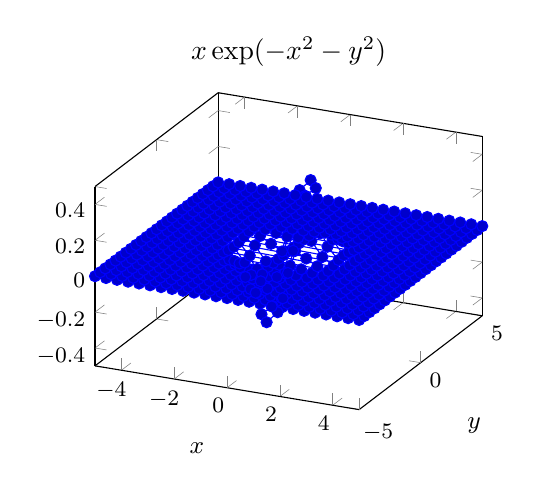
\begin{tikzpicture}
\begin{axis}[
    title={$x \exp(-x^2-y^2)$},
    xlabel=$x$, ylabel=$y$,
    small,
]
    \addplot3 {exp(-x^2-y^2)*x};
\end{axis}
\end{tikzpicture}
\end{codeexample}
%
我们的示例包含一个基本的坐标轴环境，带有前面几个教程中
已经见过的 |title|、|xlabel|、|ylabel| 和 |small| 键。
|\addplot3| 没有选项，后面紧接着就是数学表达式。
没有选项这一点告诉 \PGFPlots{} 使用它的 |cycle list|。这
进而配置了带 |blue| 颜色的 |mark=*|——以及一幅线图。
线图与 |\addplot3| 组合用处有限；它只是把所有
传入的点连接起来。由于点是以矩阵方式采样的（逐行）。我们下一步
将定义一个合适的绘图处理器。

不过注意，我们的数学表达式依赖 |x| 和 |y|。在 \PGFPlots{} 的默认
配置中，这两个变量就是采样变量：
二者都在感兴趣的 |domain| 内用正确数量的
|samples| 采样。|\addplot3| 语句负责按正确的顺序计算 $N\cdot M$ 个点，
其中 $N$ 是 $x$ 的 |samples| 数，$M$ 是
|samples y|，即 $y$ 的采样数。

我们可以看到采样 |domain| 太大。换成更小的
|domain| 可以聚焦到函数的有趣部分：

\pgfplotsexpensiveexample
\begin{codeexample}[]
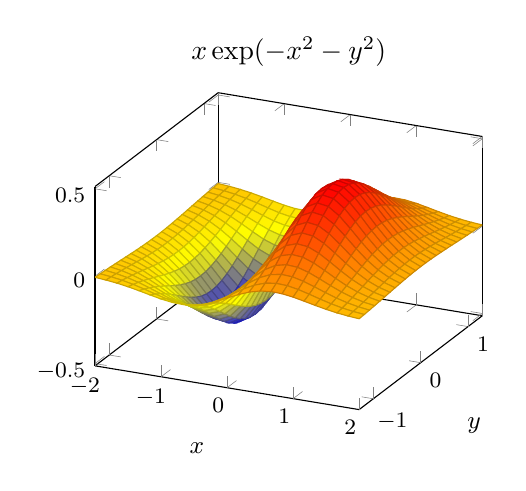
\begin{tikzpicture}
\begin{axis}[
    title={$x \exp(-x^2-y^2)$},
    xlabel=$x$, ylabel=$y$,
    small,
]
    \addplot3 [
        surf,
        domain=-2:2,
        domain y=-1.3:1.3,
    ] {exp(-x^2-y^2)*x};
\end{axis}
\end{tikzpicture}
\end{codeexample}
%
这里，我们在 |\addplot3| 之后加了一个选项列表。由于我们
提供选项列表时没有前导加号 `|+|'，\PGFPlots{}
完全不考虑它的 |cycle list|（并关闭 |mark| 和默认
颜色设置）。我们加上 |domain| 和 |domain y|，以便以合适的方式
限制采样域。如果省略 |domain y|，$y$ 域
会使用与 $x$ |domain| 相同的值。

正如你可能猜到的，|surf| 键的主要用途是与上一节教程建立
联系：它是二元函数最自然的
可视化方式之一。与上一节一样，
颜色由函数值 $z=f(x,y)$ 推出（更确切地说，
依赖默认配置 |point meta=f(x)|）。

下一步是把 `|surf|' 换成 `|contour lua|'，从而改用等高线图：

\pgfplotsexpensiveexample
\begin{codeexample}[]
\begin{tikzpicture}
\begin{axis}[
    title={$x \exp(-x^2-y^2)$},
    xlabel=$x$, ylabel=$y$,
    small,
]
    \addplot3 [
        contour lua,
        domain=-2:2,
        domain y=-1.3:1.3,
    ] {exp(-x^2-y^2)*x};
\end{axis}
\end{tikzpicture}
\end{codeexample}
%
现在，我们得到了一幅等高线图——虽然它还不完全是我们想要的。
首先，等高线太少，很难看清任何东西
（尤其是因为 |line width| 太小）。此外，|view|
方向也很陌生。

我们加上 |view| 选项，参数取“俯视”，并用
|contour/number| 键配置等高线数量，用 |thick|
样式配置 |line width|：

\pgfplotsexpensiveexample
\begin{codeexample}[]
\begin{tikzpicture}
\begin{axis}[
    title={$x \exp(-x^2-y^2)$},
    enlarge x limits,
    view={0}{90},
    xlabel=$x$, ylabel=$y$,
    small,
	colorbar,
]
    \addplot3[
        domain=-2:2,
        domain y=-1.3:1.3,
        contour lua={number=14,labels=false},
        thick,
    ] {exp(-x^2-y^2)*x};
\end{axis}
\end{tikzpicture}
\end{codeexample}

这正是我们想达到的效果。注意，|contour lua| 接受
那些键前缀为 |contour/| 的选项。在此上下文中，该前缀是
可选的。

注意，|contour lua| 在一个方面与 \PGFPlots{} 几乎所有其他绘图处理器
都不同：它要求你调用

|lualatex |\meta{texfilename}

\noindent 而不是

|pdflatex |\meta{texfilename} .

\noindent
计算等高线的非线性算法目前在 plain \TeX{} 中尚不可用，
这一点由名字 `|contour lua|' 强调。


如果你因某种原因无法使用 |lualatex|，可以把 |contour lua| 换成 |contour gnuplot|，前提是你的系统上安装了外部程序 |gnuplot|（更多细节参见 |contour gnuplot| 的参考）。

\subsection{小结}

我们勾勒了如何加载一张包含二元采样函数的数据表，并学习了
如何把这样的数据可视化为 |surf|ace 图。我们学习了如何旋转
|view|，如何改变 |surf|ace 图的颜色 |shader|，如何启用
|colorbar|，以及如何把 |scatter| 图加到曲面图之上。此外，我们以
第一幅等高线图为例，看到了如何借助 \PGFPlots{} 的内置
方法对二元函数采样。

需要强调的是，\PGFPlots{} 生成这类图不需要任何外部
工具：任何装有较新版本 \PGFPlots{} 的计算机都能重新生成这些图。

关于三维坐标轴，可讲的还有很多，尤其是
|mesh/ordering|、参数图，也许还有三维线图或
其他图类型。此外，|z buffer|ing 存在一些
局限，即 \PGFPlots{} 如何决定图的哪些部分
位于其他部分之前。这些内容可在 Section~\ref{sec:3d} 及其
小节中阅读。

你可能还对改变三维坐标轴外观的样式感兴趣，
比较 Section~\ref{sec:3d:axis:config}。

}%
